% \documentclass[a4paper, technote, draft, compsoc]{IEEEtran}
\documentclass[a4paper, technote,compsoc]{IEEEtran}
%\documentclass[a4paper]{article}

\usepackage[toc,page,titletoc]{appendix}
\usepackage[T1]{fontenc}    % use 8-bit T1 fonts
\usepackage[utf8]{inputenc} % allow utf-8 input
\usepackage{amsmath}
% \usepackage{hyperref}
\usepackage{amssymb}
\usepackage{booktabs}
\usepackage{float}  % used to fix location of images i.e.\begin{figure}[H]
\usepackage{graphicx}  %needed to include png, eps figures
\usepackage{mwe}
\usepackage{url} % correct bad hyphenation here
\usepackage[dvipsnames]{xcolor}
% \usepackage{todonotes}
\usepackage{xr}
\usepackage{subfiles}
\usepackage{physics}
\usepackage{epigraph}

\usepackage{todonotes,tocloft,xpatch,hyperref}
\hypersetup{
    colorlinks,
    linkcolor={red!50!black},
    citecolor={blue!50!black},
    urlcolor={blue!80!black}
}

% This is based on classicthesis chapter definition
\let\oldsec=\section
\renewcommand*{\section}{\secdef{\Sec}{\SecS}}
\newcommand\SecS[1]{\oldsec*{#1}}%
\newcommand\Sec[2][]{\oldsec[\texorpdfstring{#1}{#1}]{#2}}%

% https://tex.stackexchange.com/a/61267/11984
\makeatletter
\xapptocmd{\Sec}{\addtocontents{tdo}{\protect\todoline{\thesection}{#1}{}}}{}{}
\newcommand{\todoline}[1]{\@ifnextchar\Endoftdo{}{\@todoline{#1}}}
\newcommand{\@todoline}[3]{%
  \@ifnextchar\todoline
    {}
    {\contentsline{section}{\numberline{#1}#2}{#3}{}{}}%
}
\let\l@todo\l@subsection
\newcommand{\Endoftdo}{}

\AtEndDocument{\addtocontents{tdo}{\string\Endoftdo}}
\makeatother


\externaldocument[M-]{main}

\usepackage[style=ieee]{biblatex}
\bibliography{xampl}
% \usepackage[backend=biber,style=ieee]{biblatex} 
\bibliography{bibliography.bib} %your file created using JabRef

% https://tex.stackexchange.com/questions/246/when-should-i-use-input-vs-include
% \newcommand{\N}{\mathbb{N}}
\newcommand{\Z}{\mathbb{Z}}
\newcommand{\Q}{\mathbb{Q}}

\newcommand{\R}{\mathbb{R}}
\newcommand{\RR}{\mathbb{R}^2}
\newcommand{\RRR}{\mathbb{R}^3}

\renewcommand{\Pmu}{\mathcal{P}}
\renewcommand{\P}{\mathbb{P}}

\newcommand{\delt}{\Delta t}
\newcommand{\utk}{{\widetilde u}^k}
\newcommand{\ut}[1]{{\widetilde u}^{#1}}
\newcommand{\rhog}{\text{\boldmath{$\rho$}}}
\renewcommand{\eps}{\varepsilon}

\DeclareMathOperator{\sspn}{span}
\newcommand{\spn}[1]{\sspn\left(#1\right)}
\newcommand{\mytodo}[1]{\todo[inline, color=green!20, inlinewidth=\columnwidth]{#1}}

\begin{document}

\onecolumn

% paper title
\title{
    \large{(Hyper) Reduced Order Models For Moving Meshes}
    \\[5mm] Literature Review \& Research Project 
    }

% author names 
\author{Enrique Millán Valbuena \\ \normalsize{463 426 8}}% <-this % stops a space
        
% The report headers
\markboth{M. Sc. Aerospace Engineering, TU Delft}%do not delete next lines
{Shell \MakeLowercase{\textit{et al.}}: Bare Demo of IEEEtran.cls for IEEE Journals}

% make the title area
\maketitle

\begin{IEEEkeywords}
    \centering
    Finite Elements, Galerkin, Reduced Order Models, 
    Moving Piston, Deforming Mesh, ALE, 
    (M)DEIM, POD, 
    Mode Truncation
\end{IEEEkeywords}

\setcounter{tocdepth}{2}
\tableofcontents

\twocolumn

\section{Research Project}
This thesis focuses in the efficient numerical solution of parametrized unsteady PDEs with moving meshes.

Parametrized PDEs can be numerically solved with the finite element method (FEM), 
which leads to an algebraic system of equations whose solution 
can be computationally expensive to obtain, 
especially for complex geometries or elaborate models.
One refers to this FEM model as the \textit{Full Order Model}~(FOM),
\begin{equation}
   \frac{du_h}{dt} + A_h\left(t;\mu\right) u_h = f_h\left(t;\mu\right).
\end{equation}
When the problem is unsteady, that is, 
when the differential operators contain terms that change in time,
or the mesh moves in time (effectively changing the integrals of the weak form),
the algebraic operators need to be reassembled for each time step.

When this is the case, many-query procedures and access to field values or 
calculated outputs for different parameter values $\mu$ can become cumbersome, 
or even infeasible due to computational costs, both in time and memory.
To circumvent the efficiency issues, one can build a \textit{Reduced Order Model}~(ROM), 
whose solution is fast in time and light in storage.
This ROM is based in ad-hoc empirical basis functions to represent the solution, 
whose support typically spans the whole domain. 

However, due to the change in time of the operators, 
using a standalone reduced basis to represent the solution
is not enough to remove all the overheads of the FEM model.
The operators still need to be assembled 
and projected in the reduced space for each time step.
The reduced basis of the solution does shrunk the overall dimension of the system,
but it cannot remove the overhead derived from the inevitable change in the operators.
We would state to have an \textit{offline-online coupling},
since information from the FOM is required to assemble the ROM.
To overcome this issue, a system approximation technique is introduced.
We then talk about an \textit{Hyper Reduced Order Model}~(HROM).

\subsection{Outline of the Reduction Process}
The construction of the ROM has mainly two stages:
\begin{itemize}
   \item Offline stage: construction of the ROM ingredients.
   \item Online stage: assembly of the ROM to solve the PDE for unseen parametrizations.
\end{itemize}

During the offline stage, the costly algebraic problem is solved for a subset of the parameter space.
Snapshots of the matrices, vectors and solutions are stored and processed via algebraic reduction algorithms, 
in order to obtain a reduced basis for each of them.

An example of reduction algorithms would be the Discrete Empirical Interpolation Method (DEIM) 
and its matrix version (MDEIM).
These reduction algorithms need to rely on a procedure to construct the basis, 
in our case we will use the Proper Orthogonal Decomposition (POD). 

The offline stage scales with the dimension of the Full Order Model, $N_h$, 
which is governed by the number of nodes in the mesh and the polynomial degree for the FEM basis.
Once the offline stage is over, a basis for each operator of the algebraic problem has been produced, 
of representative\footnote{
   The reduction of each operator might have required a different number of basis elements, 
   but they should be all of the same order of magnitude $N \ll N_h$ or smaller for the reduction process to be a success.}
size~$N \ll N_h$.
A projection matrix $\mathbb{V}$ is derived from the solution reduced basis, 
\begin{equation}
   \mathbb{V} \in \mathbb{R}^{N_h \,\text{x}\, N}.
\end{equation} 
This matrix will be used to project once and for all 
the algebraic operator reduced basis elements, 
our HROM building blocks.
The reduced bases for the solution and the algebraic operators 
are then used during the online stage, 
where for unseen parameters a small algebraic system is built and solved,
\begin{equation}
   \frac{du_N}{dt} + A_N\left(t;\mu\right) u_N = f_N\left(t;\mu\right).
\end{equation}
At this stage, it is paramount that the assembly of the operators\footnote{
   We shall overload notation and refer to \textit{the operator} for both the matrices and the functionals,
   unless explicit distinction is required.
} 
is independent of the original problem size $N_h$.
We state to have a perfect \textit{offline-online decoupling}.

Once the reduced problem has been solved, the solution can be projected back to the original physical mesh,
\begin{equation}
   u_h = \mathbb{V} u_N.
\end{equation}
Following these steps, access to field values or calculated outputs can be obtained lightly, 
provided the overall procedure is \textit{certified}: 
to prove in the online stage that the solution is sufficiently close 
to what it would have been if the actual FOM had been assembled and solved.

All the above is presented graphically in Figure~\ref{fig:overview_graph}.

\subsection{System Approximation}
An essential ingredient to achieve a perfect \mbox{offline-online} decoupling
is what we call an \textit{
   affine decomposition} 
of the algebraic operators.
Simply put, it is to say that we can achieve a linear separation 
in the parameter, time, and spatial domains 
(the latter represented by the algebraic basis elements), 
\begin{equation}
   A_h\left(t;\mu\right) = \sum_{q=1}^{Q} \Theta_{q}(t;\mu) A_{h,q},
\end{equation}
where~$A_{h,q}$ are constant matrices referred to as the collateral basis,
and~$\Theta_{q}(t;\mu) \in \mathbb{R}$ are scalar values. 

The easiest example one could come up with of an affine decomposition is the one present 
in the heat diffusion problem with two different but uniform diffusion parameters $k_q$ across the domain.
The affine decomposition would look like
\begin{equation}
   A_h\left(t;k_1, k_2\right) = k_{1} A_{h,1} + k_{2} A_{h,2},
\end{equation}
where each matrix $A_{h,q}$ would represent the diffusion operator with support over the subdomain associated with each parameter. 
For this simple example, the affine decomposition is present naturally within the PDE structure, 
but this will not always be the case, specially when nonlinearities are present. 

However, nowadays it is absolutely possible to obtain an automatic ad-hoc affine decomposition 
for any operator thanks to grounded algorithms and procedures, like DEIM and MDEIM.
This key fact will allows us to achieve a perfect split between the offline and the online stage, 
as it will allow us to assemble our ROM operators without having to assemble at any point the complete FOM operator. 

\subsubsection{Nonlinear Term Reduction}
The reduction of a nonlinear term can be achieved 
with the same MDEIM technique as the one used for linear operators.

The only difference is that the coefficient functions~$\Theta_{q}$ from 
the affine decomposition depend on the solution values too,
\begin{equation}
   A_h\left(t;\mu\right, u) = \sum_{q=1}^{Q} \Theta_{q}(t;\mu, u) A_{h,q}.
\end{equation}
Nevertheless, this fact does not necessarily break the convergence and approximation 
properties derived for MDEIM,
so we expect to use it successfully.   

% Ideally, 
%% Research objectives
% Useful: benefit of your research to the problem. 
% Realistic: contribute to the solution of the problem.
% Feasible: time scheduled and capabilities and resources.
% Clear: be precise in the contribution to the problem.
% Informative: rough idea of knowledge generated towards a solution.

% The research objective is (a) by (b).
% (a) The contribution of the research project to the solution of the problem.
% (b) description of the way the contribution will be provided. 

\subsubsection{Implicit \textit{Nonlinearities}}
A nonlinearity can be seen essentially as a characteristic that prevents a linear separation.
Despite the apparent linear character of an algebraic equation, 
from the point of view of the affine decomposition, 
it could potentially hide a nonlinearity.

The introduction of the time variable~$t$~in the shape of the mesh makes it so
that the operators change at each time step during the integration loop.
Additionally, since the domain geometry will depend on some parameter values too, 
one cannot explicitly write the affine decomposition of the operators in a closed form.
This is implicitly collected by the Jacobian,
the transformation that maps integrals over moving meshes 
to one over a reference fixed mesh.

Another type of nonlinearity would be a term whose integrand contained 
a nonlinear function applied over the $u$ field,
or interactions of the solution with its own derivatives.
% These kind of non-linearities are common in mathematical modelling, 
% but shall keep out of the scope of this work to keep a narrow focus. 
% The non-linearity of the basic operators will give us enough work already.

\subsection{Kick-off Point}
The (M)DEIM reduction technique have been successfully used with domains
whose boundary is parametrized, but whose mesh remained fixed in time \cite{Santo_Manzoni_2019}. 

We aim at extending these results by introducing a moving mesh in time,
thus allowing us to obtain an hyper reduced order model which can tackle 
more complex \mbox{real-life} problems.
The additional complexities introduced by the moving mesh are the introduction 
of the Arbitrary Eulerian Lagrangian formulation (ALE), 
and the increase in the number of operator snapshots to be collected during the offline stage.  

\onecolumn
\begin{figure}[h]
   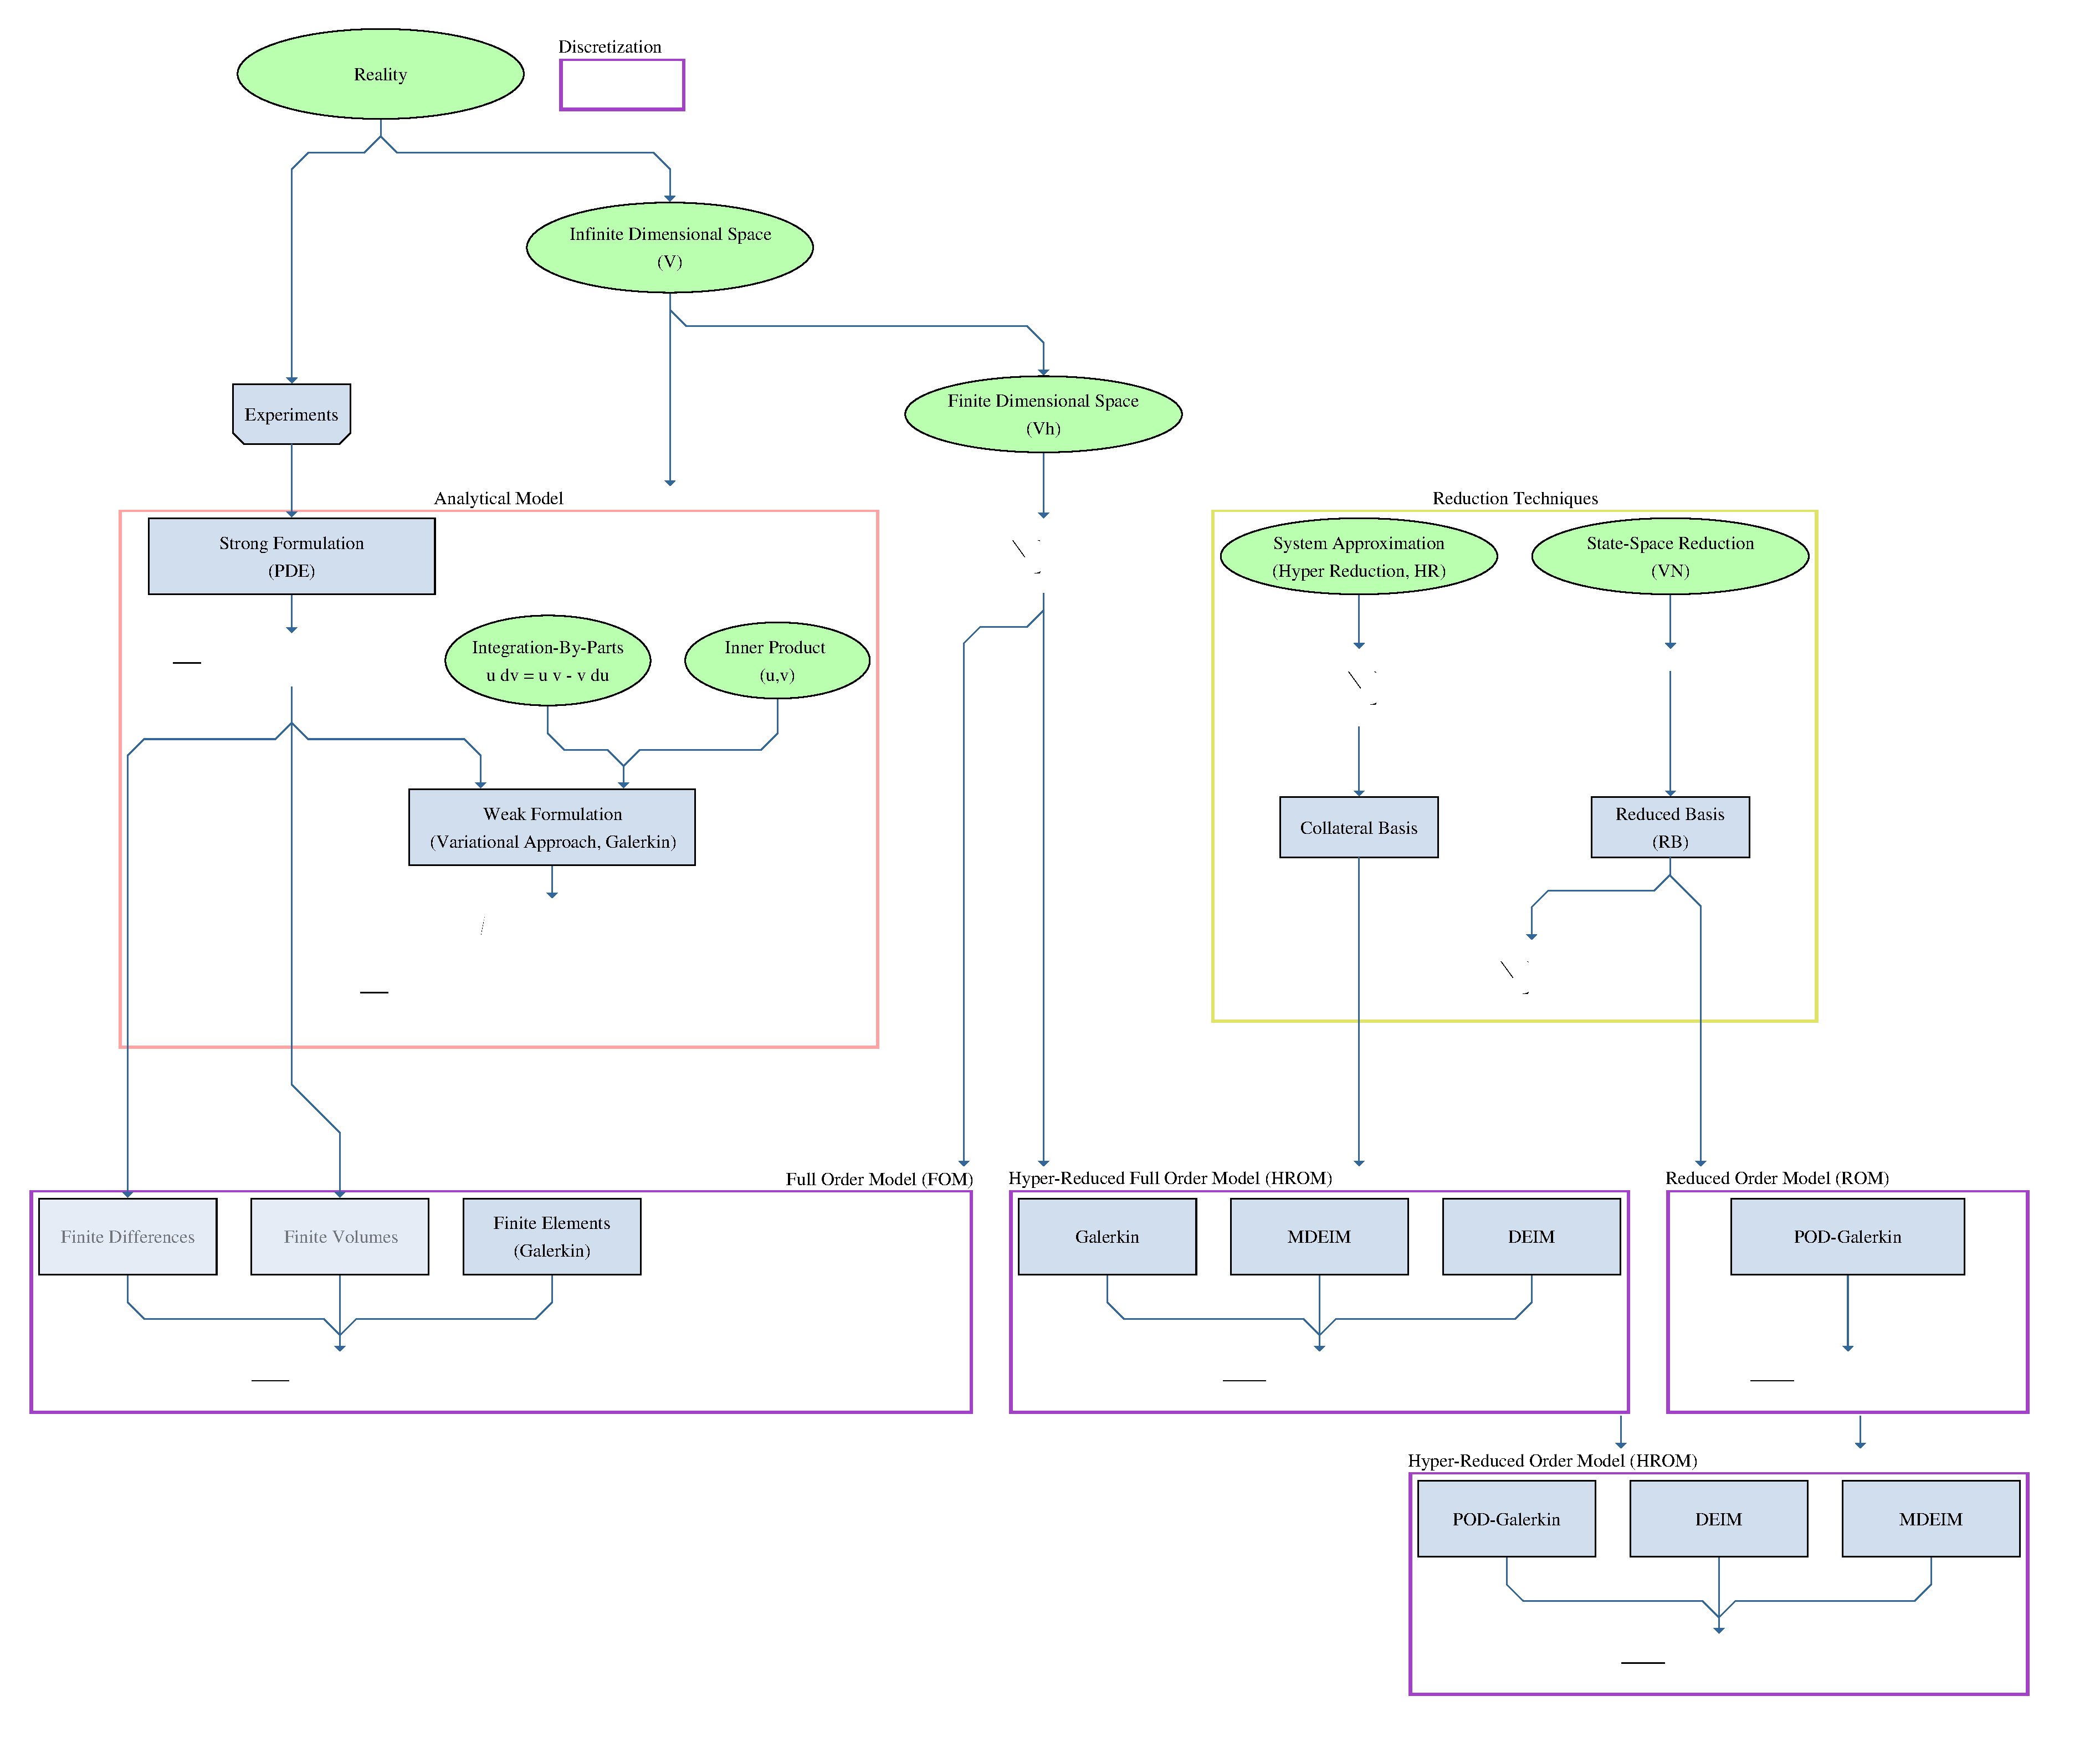
\includegraphics[width=\columnwidth]{graphs/From-Reality-To-ROM.png}
   \caption{Building blocks of the transition from reality to discrete 
   reduced order modeling.
   On the left side we present the traditional finite element course: 
   from the observation of reality a parametrized PDE model is derived 
   (infinite dimensional space, unknown analytical solution).
   The paremeters allow the model to capture a range of 
   boundary conditions, geometries,
   and term-domination effects, 
   all of them driven by the same physics.
   % 
   This model can be cast into a weak form and 
   solved numerically via the Galerkin projection 
   (finite dimensional space, Lagrangian piecewise solution).
   The finite element method is a robust and well-established technique
   for the solution of parametrized PDEs.
   However, for three-dimensional domains, 
   or complex modelling terms, the algebraic operators involved (vectors and matrices) 
   can become computationally expensive to assemble and solve,
   especially for unsteady problems with moving meshes.
   % 
   On the right side, we present two reduction techniques introduced 
   to increase the efficiency of the numerical solution:
   the construction of a \textit{reduced basis} (RB), also known as state-space reduction;
   and the determination of a collateral basis for 
   the algebraic finite element operators, known as \textit{system approximation}.
   The reduced basis is used in substitution of the Lagrangian piecewise functions,
   the collateral basis is used to skip the assembly 
   of all the entries of each algebraic operator.
   % 
   All in all, the simultaneous use of these two reduction techniques 
   leads to an algebraic hyper-reduced order model,
   cheaper to assemble and solve than the traditional finite element problem;
   and for problems with time-dependent matrices,
   even cheaper than assembling the operators and projecting them
   unto the reduced basis for each time step.}
   \label{fig:overview_graph}
 \end{figure}
 \twocolumn

\section{Literature Review}
%% Lab Report for EEET2493_labreport_template.tex
%% V1.0
%% 2019/01/16
%% This is the template for a Lab report following an IEEE paper. Modified by Francisco Tovar after Michael Sheel original document.


%% This is a skeleton file demonstrating the use of IEEEtran.cls
%% (requires IEEEtran.cls version 1.8b or later) with an IEEE
%% journal paper.
%%
%% Support sites:
%% http://www.michaelshell.org/tex/ieeetran/
%% http://www.ctan.org/pkg/ieeetran
%% and
%% http://www.ieee.org/

%%*************************************************************************
%% Legal Notice:
%% This code is offered as-is without any warranty either expressed or
%% implied; without even the implied warranty of MERCHANTABILITY or
%% FITNESS FOR A PARTICULAR PURPOSE! 
%% User assumes all risk.
%% In no event shall the IEEE or any contributor to this code be liable for
%% any damages or losses, including, but not limited to, incidental,
%% consequential, or any other damages, resulting from the use or misuse
%% of any information contained here.
%%
%% All comments are the opinions of their respective authors and are not
%% necessarily endorsed by the IEEE.
%%
%% This work is distributed under the LaTeX Project Public License (LPPL)
%% ( http://www.latex-project.org/ ) version 1.3, and may be freely used,
%% distributed and modified. A copy of the LPPL, version 1.3, is included
%% in the base LaTeX documentation of all distributions of LaTeX released
%% 2003/12/01 or later.
%% Retain all contribution notices and credits.
%% ** Modified files should be clearly indicated as such, including  **
%% ** renaming them and changing author support contact information. **
%%*************************************************************************

% \documentclass[a4paper, technote, compsoc]{IEEEtran}
\documentclass[../main.tex]{subfiles}

% \usepackage[T1]{fontenc}    % use 8-bit T1 fonts
% \usepackage[utf8]{inputenc} % allow utf-8 input
% \usepackage{amsmath}
% \usepackage{amssymb}
% \usepackage{booktabs}
% \usepackage{float}  % used to fix location of images i.e.\begin{figure}[H]
% \usepackage{graphicx}  %needed to include png, eps figures
% \usepackage{mwe}
% \usepackage{subfiles}
% \usepackage{url} % correct bad hyphenation here
% \usepackage{xcolor}

% \usepackage[backend=biber,style=ieee]{biblatex} 
% \bibliography{biblio.bib} %your file created using JabRef

\begin{document}

% % paper title
% \title{Reduced Order Models \\ With Moving Domains \\ \normalsize{Literature Review}}

% % author names 
% \author{Enrique Millán Valbuena \\ \normalsize{463 426 8}}% <-this % stops a space
        
% % The report headers
% \markboth{M. Sc. Aerospace Engineering, TU Delft}%do not delete next lines
% {Shell \MakeLowercase{\textit{et al.}}: Bare Demo of IEEEtran.cls for IEEE Journals}

% % make the title area
% \maketitle

% % As a general rule, do not put math, special symbols or citations
% % in the abstract or keywords.
% \begin{abstract}
% TBD
% \end{abstract}

% \begin{IEEEkeywords}
% Reduced basis methods, moving domain, heat equation, Galerkin-projection, FEM, DEIM, MDEIM, POD
% \end{IEEEkeywords}

\section{Introduction}

From  \cite{2016_CertifiedReducedBasisMethodsParametrizedPDE_Hesthaven}:
\begin{quotation}
    The central idea of the reduced basis approach is the identification of a suitable problem-dependent basis to effectively represent parametrized solutions to partial differential equations.
\end{quotation}

\begin{itemize}
    \item Difference between local and global support.
    \item Decomposition techniques.
\end{itemize}

\section{Needs}
We aim at obtaining efficiently the solution of parametrized parabolic PDEs with moving boundaries in time.

\begin{itemize}
    \item Build a ROM system equivalent to the FEM discretization of the weak form of the PDE.
    \begin{itemize}
        \item Solve the ROM for each time-step and project back to physical domain.
        \item Functional evaluation of the solution.
    \end{itemize}
    \item Do not assemble and project any high fidelity operators to build the ROM operators.
    \begin{itemize}
        \item Sampling strategies across the parameter space are crucial.
            \begin{itemize}
                \item Ensure convergence.
                \item Computational efficiency.
            \end{itemize}
        \item Create a POD-basis for:
        \begin{itemize}
            \item The solution space.
            \item Each operator, matrix or vector, of the system.
            \item How does the selection of the inner product change the resultant basis of the POD?
            \item Can we use information from the PDE to improve this inner product?
            \item Why does the POD generate basis functions with global support? 
        \end{itemize}
        \item Discrete Empirical Interpolation of the ROM operators.
        \item Greedy sampling techniques are similar in objective to, but very different in approach from, the more well-known methods of proper orthogonal decomposition (POD). How are they different?
    \end{itemize}
    \item Certify the ROM solution with a posteriori error bounds.
\end{itemize}

\subsection{Scope}
\begin{itemize}
    \item Prescribed deformation of the domain:
    \begin{itemize}
        \item Interpolate through the mesh with a Laplacian operator for each time-step.
        \item Separable geometrical and time parametrization of the domain deformation.
        \item No FSI problem to be solved.
    \end{itemize}
    \item Linear operators:
    \begin{itemize}
        \item Heat equation.
        \item Convection-diffusion with known velocity field. 
    \end{itemize}
    \item Lifting function for boundary conditions:
    \begin{itemize}
        \item The homogeneous problem is reduced.
        \item The lifting operators are reduced. 
    \end{itemize}
\end{itemize}
\section{What Others Have Done}
\begin{itemize}
    \item POD-Galerkin projection.
    \item Operators reduction:
    \begin{itemize}
        \item (DEIM) Vector reduction and interpolation \cite{2010_nonlinearModelReductionDeim_chaturantabut}.
        \item (MDEIM) Matrix reduction and interpolation \cite{2015_efficientModelReductionParametrizedSystemsMatrixDeim_Negri}.
        \item Reduction of non-linear operators.
    \end{itemize}
    \item Problem parametrization: 
    \begin{itemize}
        \item PDE coefficients.
        \item Boundary conditions.
        \item Geometrical deformation of the domain.
    \end{itemize}
\end{itemize}

\section{What We Intend To Do}

\subsection{Research Questions}

\begin{itemize}
    \item How does the parameter sampling strategy affect the goodness of the POD-basis?
    \item How does the parameter sampling strategy affect the goodness of the Discrete Empirical Interpolation?
    \item Can we predict the minimum viable number of basis for a given error?
    \item What is a representative snapshot?
    \item When can we consider the basis sufficiently rich?
    \item What does it mean for a basis to be \textit{rich}? 
\end{itemize}

\section{Conclusions}
\label{sec:conclusions}

\printbibliography

\end{document}




\newpage
\section{Plan and Scope}
%% Lab Report for EEET2493_labreport_template.tex
%% V1.0
%% 2019/01/16
%% This is the template for a Lab report following an IEEE paper. Modified by Francisco Tovar after Michael Sheel original document.


%% This is a skeleton file demonstrating the use of IEEEtran.cls
%% (requires IEEEtran.cls version 1.8b or later) with an IEEE
%% journal paper.
%%
%% Support sites:
%% http://www.michaelshell.org/tex/ieeetran/
%% http://www.ctan.org/pkg/ieeetran
%% and
%% http://www.ieee.org/

%%*************************************************************************
%% Legal Notice:
%% This code is offered as-is without any warranty either expressed or
%% implied; without even the implied warranty of MERCHANTABILITY or
%% FITNESS FOR A PARTICULAR PURPOSE! 
%% User assumes all risk.
%% In no event shall the IEEE or any contributor to this code be liable for
%% any damages or losses, including, but not limited to, incidental,
%% consequential, or any other damages, resulting from the use or misuse
%% of any information contained here.
%%
%% All comments are the opinions of their respective authors and are not
%% necessarily endorsed by the IEEE.
%%
%% This work is distributed under the LaTeX Project Public License (LPPL)
%% ( http://www.latex-project.org/ ) version 1.3, and may be freely used,
%% distributed and modified. A copy of the LPPL, version 1.3, is included
%% in the base LaTeX documentation of all distributions of LaTeX released
%% 2003/12/01 or later.
%% Retain all contribution notices and credits.
%% ** Modified files should be clearly indicated as such, including  **
%% ** renaming them and changing author support contact information. **
%%*************************************************************************

\documentclass[a4paper, technote, compsoc]{IEEEtran}
% \documentclass{article}

% *** CITATION PACKAGES ***
\usepackage[backend=biber,style=ieee]{biblatex} 
\bibliography{biblio.bib}
   %your file created using JabRef

% *** MATH PACKAGES ***
\usepackage{amsmath}

% *** PDF, URL AND HYPERLINK PACKAGES ***
\usepackage{url}
% correct bad hyphenation here
\usepackage{graphicx}  %needed to include png, eps figures
\usepackage{float}  % used to fix location of images i.e.\begin{figure}[H]

\usepackage[utf8]{inputenc} % allow utf-8 input
\usepackage[T1]{fontenc}    % use 8-bit T1 fonts
\usepackage{xcolor}
\usepackage{booktabs}
\usepackage{mwe}

\begin{document}

% paper title
\title{Reduced Order Models \\ With Moving Domains \\ \normalsize{Research Project}}

% author names 
\author{Enrique Millán Valbuena \\ \normalsize{463 426 8}}% <-this % stops a space
        
% The report headers
\markboth{M. Sc. Aerospace Engineering, TU Delft}%do not delete next lines
{Shell \MakeLowercase{\textit{et al.}}: Bare Demo of IEEEtran.cls for IEEE Journals}

% make the title area
\maketitle

% As a general rule, do not put math, special symbols or citations
% in the abstract or keywords.
\begin{abstract}
   TBD
\end{abstract}

\begin{IEEEkeywords}
Reduced basis methods, moving domain, heat equation, FEM, DEIM, MDEIM, POD, Galerkin-projection
\end{IEEEkeywords}

\section{Introduction}
\section{Introduction}

\newpage
\section{Conclusions}
\label{sec:conclusions}

\printbibliography

% http://danceswithcode.net/engineeringnotes/rotations_in_3d/rotations_in_3d_part1.html

\end{document}




\newpage
\printbibliography

\end{document}